\documentclass[journal]{journal}
%\usepackage[tight,footnotesize]{subfigure}
\usepackage{subcaption}
\usepackage{graphicx}
\usepackage{url}
\usepackage{color}
\usepackage{multirow}
\usepackage{makecell}
%define some own functions
\newcommand{\tabincell}[2]{\begin{tabular}{@{}#1@{}}#2\end{tabular}} 

% correct bad hyphenation here
\hyphenation{op-tical net-works semi-conduc-tor}
\pagestyle{empty}
\begin{document}

\title{Real-Time Hand Posture Recognition on a Neuromorphic System}
\author{
Qian~Liu, 
and~Steve~Furber,~\IEEEmembership{Fellow,~IEEE}
\thanks{
The authors are with the School of Computer Science, University of Manchester, Manchester M13 9PL, U.K. 
(e-mail:liuq@cs.man.ac.uk; steve.furber@manchester.ac.uk).}
}% <-this % stops a space
%\thanks{Manuscript received April 19, 2005; revised January 11, 2007.}}

\maketitle
\thispagestyle{empty}

\begin{abstract}
%\boldmath
In order to make an effective, energy-efficient touch-less user interface (UI), we modelled an optimized spiking neural network (SNN) based hand-gesture command identifier on bespoke hardware. 
Goal 1:  prototype a neural gesture recognition system on SpiNNaker. 
Once the gesture recognition system is functioning effectively the SpiNNaker platform can then be used to explore the optimal spiking neural network size and configuration for the gesture recognition task.
Goal 2:  evaluate the cost and performance trade-offs in optimizing the number of neural components required to deliver effective gesture recognition.
\end{abstract}

\begin{IEEEkeywords}
spiking neural network (SNN), convolutional neural network (CNN), posture recognition, neuromorphic system.
\end{IEEEkeywords}

\section{Introduction}
\IEEEPARstart{A} pattern or an object in a two-dimensional image can be described with four properties~\cite{wysoski2008fast}: position, geometry (size, area and shape), color and texture, and trajectory. Appearance-based methods are the most direct approaches to perform pattern recognition. 
The test image is compared with all the templates to find the best match on one particular or a combination of properties. 
In terms of classification algorithms, distance measure methods (nearest neighbour, k-means clustering), support vector machine (SVM), multi-layer perceptron (MLP) neural networks and statistical methods, e.g. Gaussian mixture model (GMM) have been applied successfully in visual recognition. 
Since the 2D projection of an object changes under various illuminations, viewing angles, relative positions and distances (size), it is impossible to represent all appearances of an object in different conditions. 
Robust matching methods are employed, such as edge matching~\cite{canny1986computational}, the divide-and-conquer approach~\cite{toygar2004multiple}, gradient matching~\cite{wei2006robust}, etc. 
Moreover, feature based methods are used to improve reliability, robustness and classification efficiency. 
Among various feature extraction methods, the scale-invariant feature transform (SIFT)~\cite{lowe2004distinctive} and the sped-up robust features (SURF)~\cite{bay2008speeded} methods are well-accepted recently in the field. 
However, to find a proper feature for a specific object still remains an open question and there is not any process as accurate, general and effective as the brain.
Turning to biology for answers is always the way to explore the field of visual pattern recognition. 
Riesenhuber and Poggio~\cite{riesenhuber1999hierarchical} presented a biologically-inspired model following the organization of the visual cortex which has the ability to represent relative position- and scale-invariant features. Integrating a rich set of visual features became available using a feed-forward hierarchical pathway. 

More and more attention has been drawn into the investigation of spiking neural networks for vision processing. 
Pattern information can be encoded in the delays between the pre- and post-synaptic spikes since the spiking neurons are capable of computing radial basis functions (RBFs)~\cite{hopfield1995pattern}.  
A further study~\cite{natschlager1998spatial} has stated that spatio-temporal information can be also stored in the exact firing time instead of the relative delay. Maass~\cite{maass1997networks} has proved mathematically that:
1) networks of spiking neurons are computationally more powerful than the first and second generation of neural network models;
2) a concrete biologically relevant function can be computed by a single spiking neuron, replacing  hundreds of hidden units in a sigmoidal neural net;
3) any function that can be computed by a small sigmoidal neural net can also be computed by a small network of spiking neurons.
Applications of SNN-based vision processing have been successfully carried out. 
A two-layered SNN has been trained using spike time dependent plasticity (STDP) and employed for a character recognition task~\cite{gupta2007character}. 
Lee and co-authors~\cite{6467270} have implemented the direction selective filters in real time using spiking neurons. 
The direction selective filters here are considered as a layer of convolution module in the model of so called convolution neural network~\cite{camunas2012event}. 
Different features, such as Gabor filter features (scale, orientation and frequency) and shape can be modelled as layers of feature maps. 
Rank order coding, as an alternative to conventional rate-based coding, treats the first spike the most important and has well applied to an orientation detection training process~\cite{delorme2001networks}. 
Nengo~\cite{eliasmith2011nengo} is a graphical and scripting based software package for simulating large-scale neural systems and has been used to build the world's largest functional brain model, Spaun~\cite{eliasmith2012large}. An FPGA implementation of a Nengo model for digit recognition has been reported~\cite{naylor2013managing}. 
Deep Belief Networks (DBNs), the 4th generation of artificial neural network, has shown a strong ability in solving classification problems. 
A recent study~\cite{o2013real} has resoundingly mapped an offline-trained DBN onto an efficient event-driven spiking neural network for a digit recognition task.
Hand segmentation and feature extraction usually takes the colour into account and involves wavelets, e.g. using a Kalman filter. 
Thus, shape-only recognition of the hand posture will be a challenge. 
In the terms of gesture recognition, the hidden Markov model (HMM) has shown its ability to recognize dynamic gestures~\cite{elmezain2009hidden}. 
However, with their instinctive temporal processing, SNNs have the potential to deliver dynamic gesture recognition.

\section{Neuromorphic Platform}
\textcolor{blue}{
This section presents some details of the two hardware components, the Address-Event Representation (AER) silicon retina~\cite{lenero20113} and the SpiNNaker system~\cite{furber2014spinnaker} which is a massive parallel computing platform aimed at real-time simulation of spiking neural networks (SNNs). 
Figure~\ref{fig:SysOverView} shows the combined hand posture recognition system; 
the AEREAR2 silicon retina connected to the SpiNNaker 48-node board via a Spartan 6 FPGA board~\cite{galluppi2012real}.%, which was also applied to a sound localisation system.
The jAER~\cite{delbruck2008frame} event-based processing software\footnote{\url{http://sourceforge.net/p/jaer/wiki/Home/}} running on the PC configures the retina and displays the output spikes through a USB link.
The host communicates to the SpiNNaker board via Ethernet to set up its runtime parameters and to download the neural network model off-line and uses a visualiser~\cite{6252490} to show the spiking activities in real-time.
}

\begin{figure}
\centering
	\begin{subfigure}[t]{0.42\textwidth}
		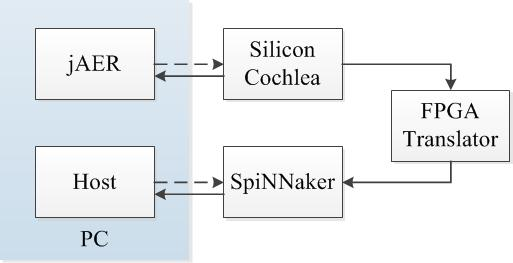
\includegraphics[width=\textwidth]{pics/outline.jpg}
	    \caption{Outline of the platform}
	    \label{fig:SysOverViewa}
	\end{subfigure}
	\\
	\begin{subfigure}[t]{0.42\textwidth}
		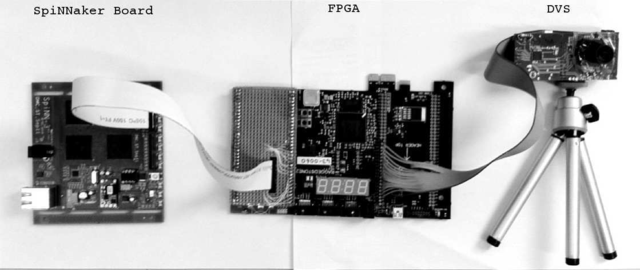
\includegraphics[width=\textwidth]{pics/dvs_spinnaker.png}	    \caption{Picture of the hardware platform}
	    \label{fig:SysOverViewb}
	\end{subfigure}	

\caption{System overview of the posture recognition platform. The silicon retina connects to the SpiNNaker system through an FPGA board. 
Spikes from the retina are streamed to the SpiNNaker system through this Spartan-6 FPGA board.
The jAER software configures the retina and displays its outgoing spikes through the USB connection.
The host sets up the runtime parameters off-line and downloads the network model to the SpiNNaker system.
}
\label{fig:SysOverView}
\end{figure}

\subsection{Silicon Retina}
\textcolor{blue}{
The visual front-end is constituted by a Dynamic Video Sensor (DVS) silicon retina, an asynchronous sensor which provides spike events encod-
ing the address of pixels undergoing a contrast change\cite{wei2006robust}. 
This approach lies in opposition to the more traditional method of sending entire frames to provide fast (3 $\mu$s latency) data-driven contrast detection at a wide range of illuminations. 
The sensor is capable of transmitting from 1 Keps to 20 Meps (events per
second).}

\subsection{SpiNNaker System}
The SpiNNaker project's architecture mimics the human brain's biological structure and functionality. 
This offers the possibility of utilizing massive parallelism and redundancy to provide resilience in an environment of unreliability and failure of individual components.

In the human brain, communication between its computing elements, or neurons, is achieved by the transmission of electrical "spikes" along connecting axons. 
The biological processing of the neuron can be modelled by a digital processor and the axon connectivity can be represented by messages, or information packets, transmitted between a large number of processors which emulate the parallel operation of the billions of neurons comprising the brain.

The engineering of the SpiNNaker concept is illustrated in the Figure~\ref{fig:sysdia} where the hierarchy of components can be identified. 
Each element of the toroidal interconnection mesh is a multi-core processor known as the "SpiNNaker Chip" comprising 18 processing cores. 
Each core is a complete processing sub-system with local memory and a DMA capability. 
It is connected to its local peers via a Network-on-Chip (NoC) which provides local high bandwidth communication and to other SpiNNaker chips via links between SpiNNaker chips. 
In this way the massive parallelism extending to thousands or millions of processors is possible.

\begin{figure}
\centering
	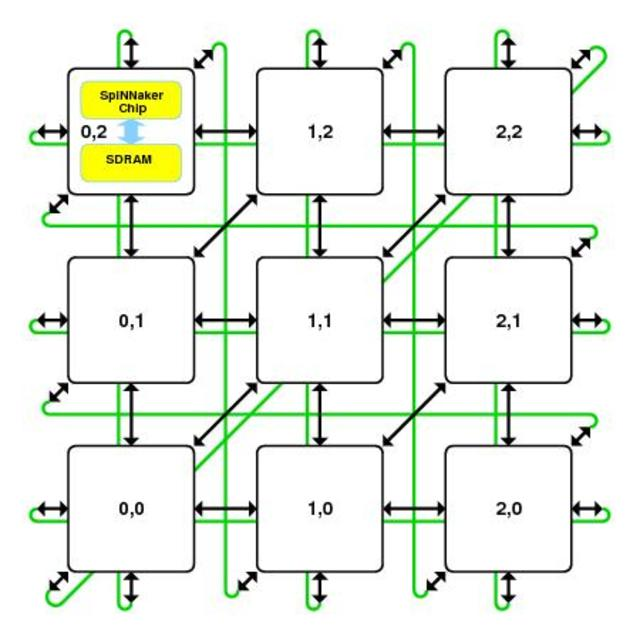
\includegraphics[width=0.42\textwidth]{pics/mesh_ctiff.jpg}
	\caption{System diagram}
	\label{fig:sysdia}
\end{figure}

The knowledge content and learning ability of the brain is embodied in its evolvable interconnection pattern; 
this routes a spike generated by one neuron to others which are interconnected with it by axons and these interconnections are modified and extended as a result of the learning and processes.

In SpiNNaker a packet Router within each multi-core processor controls the neural interconnection. 
Each transmitted packet representing a spike contains information which identifies its source neuron; 
this is used by a multi-core processor's Router to identify whether this packet should be routed to one of its contained application processors to respond, or should be routed on to one of the six adjacent multi-core processors connected to it as part of the overall SpiNNaker network.

The 103 machine is the 48-node board, see Figure~\ref{fig:48node}, and has 864 ARM processor cores, typically deployed as 768 application cores, 48 Monitor Processors and 48 spare cores. The 103 machine requires a 12V 6A supply. 
The control interface is two 100Mbps Ethernet connections, one for the Board Management Processor and the second for the SpiNNaker array. 
There are options to use the nine on-board 3.1Gbps high-speed serial interfaces (using SATA cables, but not necessarily the SATA protocol) for I/O; 
this will require suitable configuration of the on-board FPGAs that provide the high-speed serial interface support. 
103 boards can be connected together to form larger systems using the high-speed serial interfaces. 

\begin{figure}
\centering
	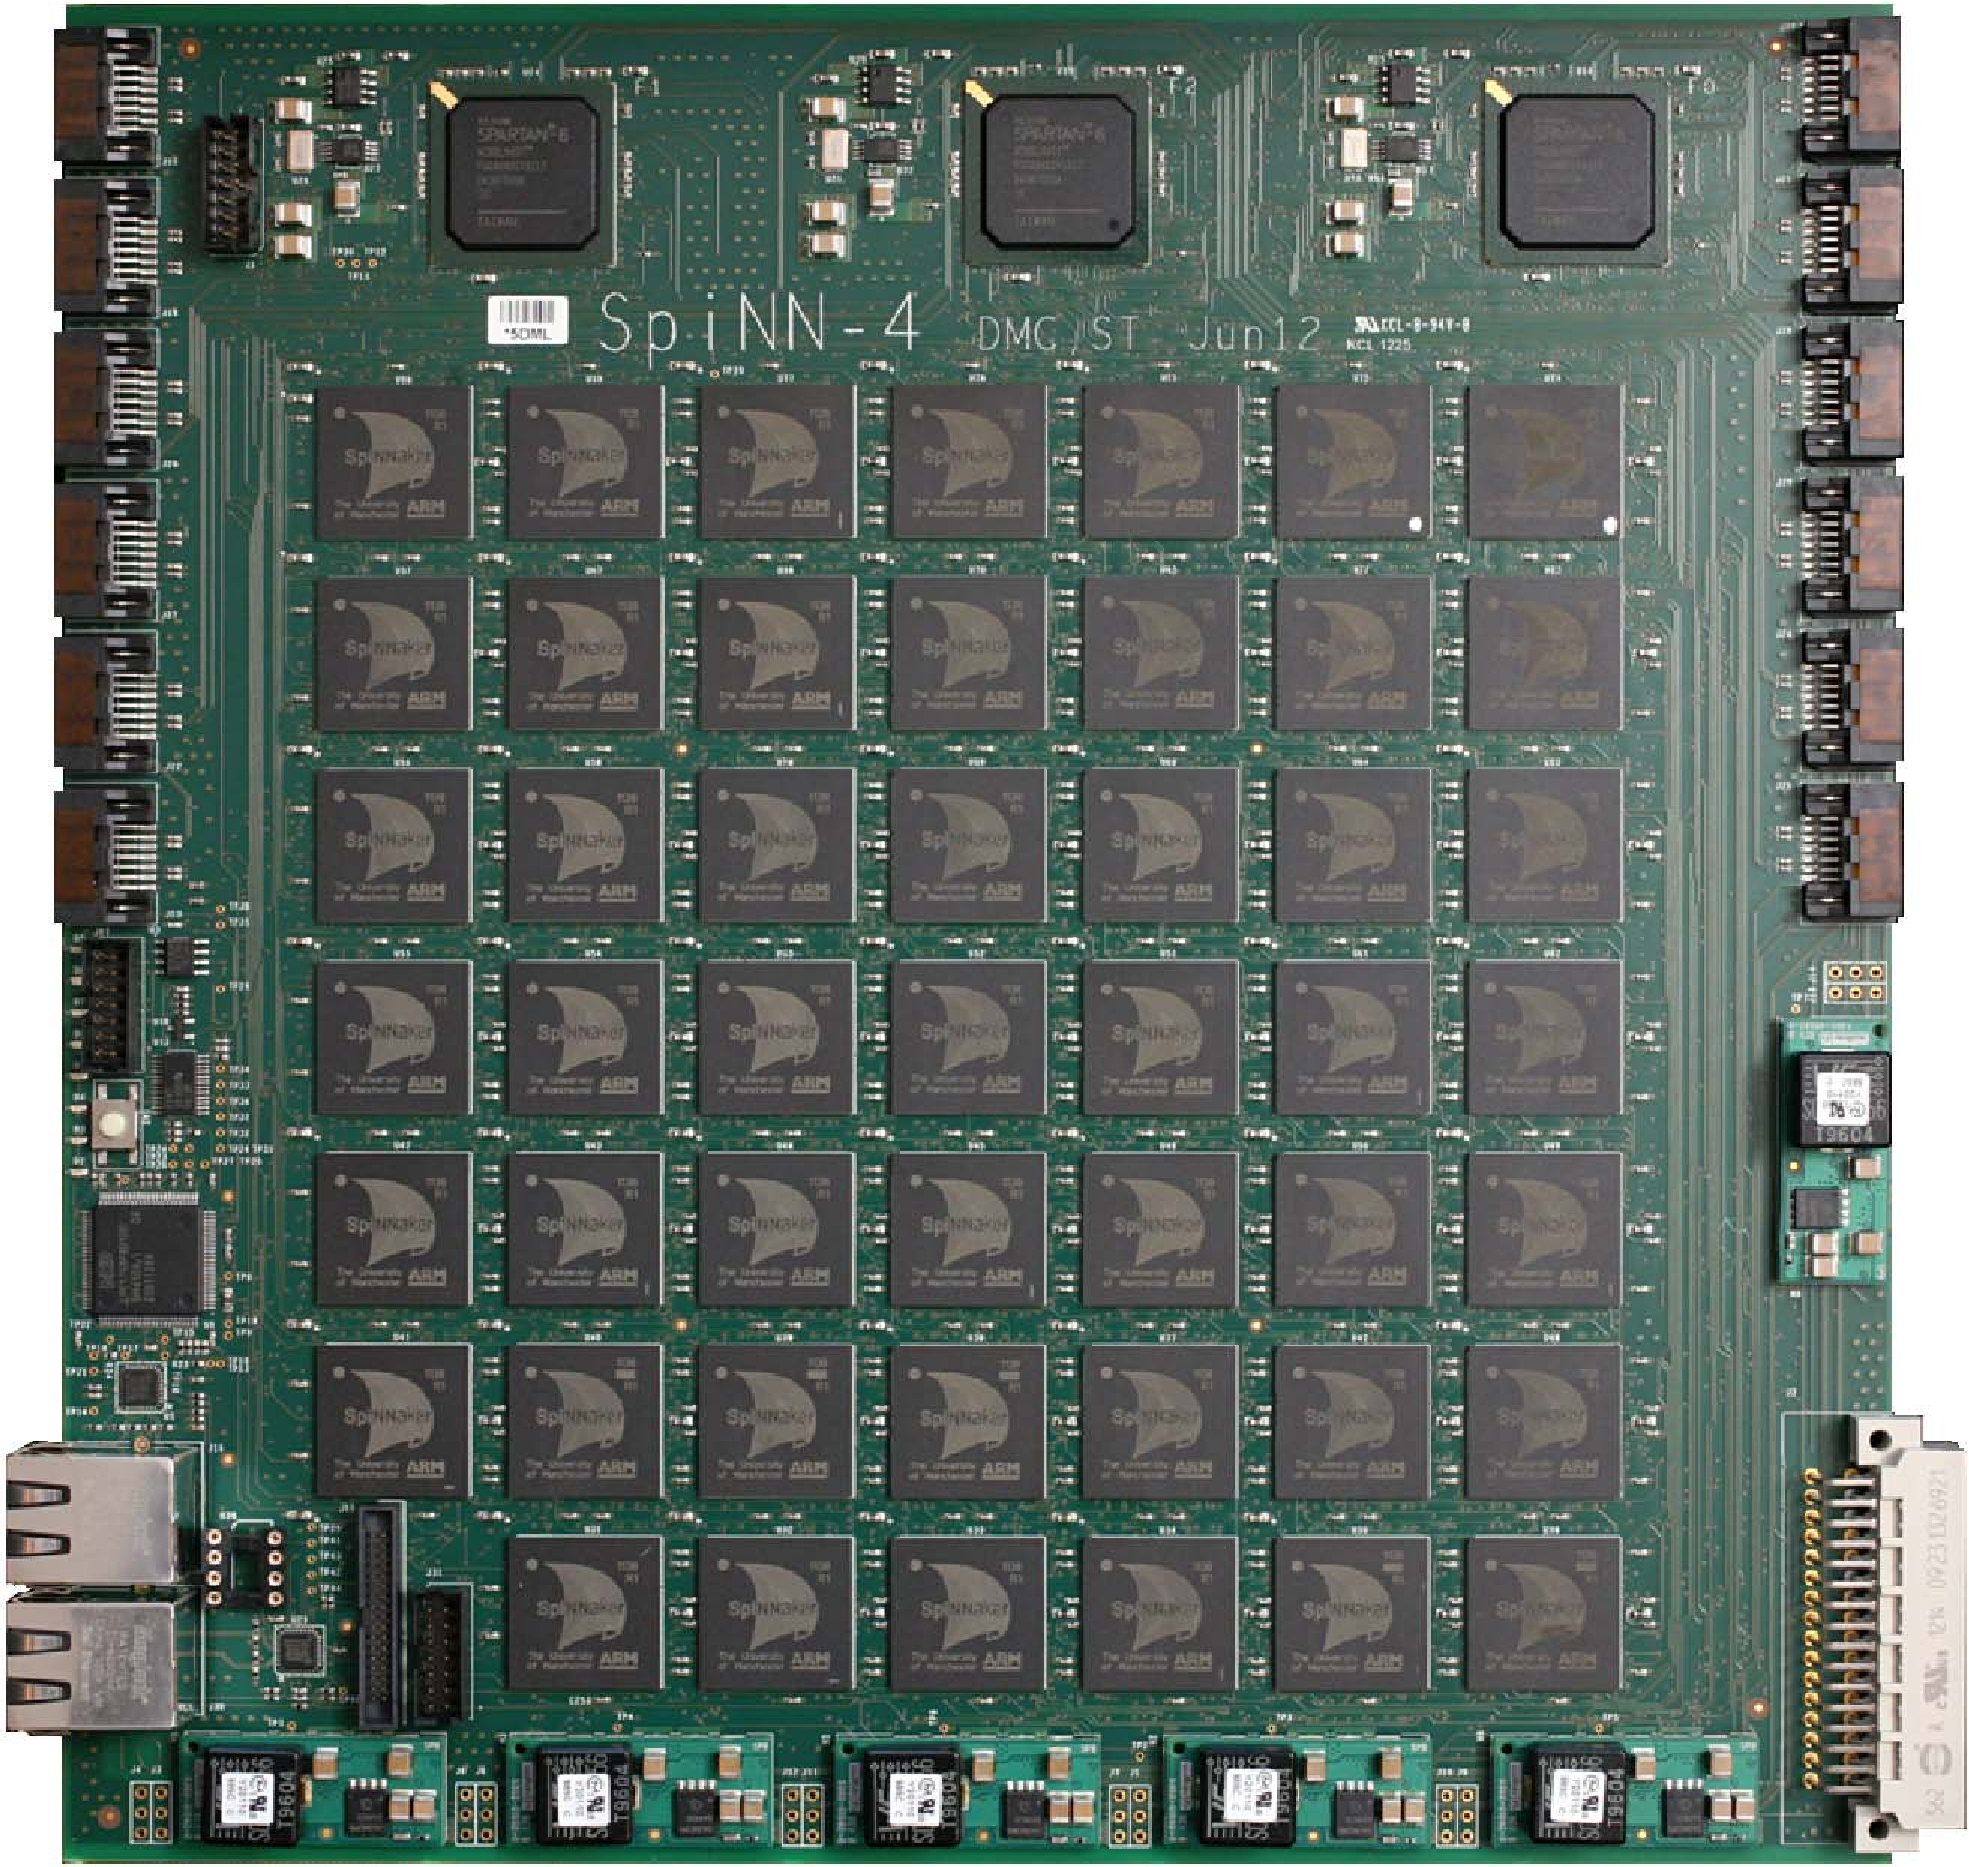
\includegraphics[width=0.42\textwidth]{pics/48node_pcb_resolution-white.pdf}
	\caption{103 Machine PCB}
	\label{fig:48node}
\end{figure}

\subsection{Interfacing AER Sensors}
Spikes from the silicon retina are injected to SpiNNaker through one of the 6 bi-directional on-board links by a SPARTAN-6 FPGA board that translates them into a SpiNNaker compatible AER format \footnote{AppNote 8 - Interfacing AER devices to SpiNNaker using an FPGA.}. 
From the software point of view, interfacing the silicon retina can be done using pyNN. 
The user sets a Spike Source population that resides on a virtual SpiNNaker chip, to which an AER sensor's spikes are directed, thus abstracting away the hardware details from the users\cite{galluppi2012real}.

\section{Convolutional Neural Networks}
\label{sec:cnn}
The convolutional neural network (CNN) is well-known as an example of a biologically-inspired model. 
The repeated convolutional kernels are overlapped in the receptive fields of the input neurons. 
Figure~\ref{fig:conv} shows a typical convolutional connection between two layers of neurons. 

\begin{figure}
\centering
	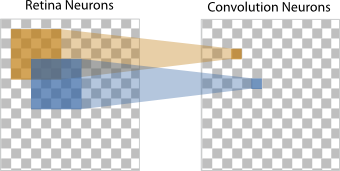
\includegraphics[width=0.42\textwidth]{pics/convolution.png}
	\caption{Each individual convolution neuron connects to its respective field using the same kernel.}
	\label{fig:conv}
\end{figure}

\subsection{Model Description}
\label{sec:mds}
There are two CNNs proposed to accomplish the posture recognition task.
A straight forward method of template matching was employed at first, and then a multi-layer perceptrons (MLP) was trained to improve the recognition performance.
\subsubsection{Manual Feature Extraction Model}

\begin{figure}
\centering
	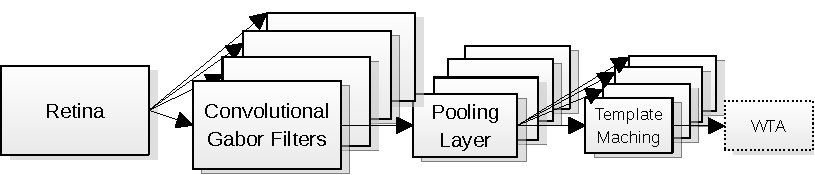
\includegraphics[width=0.42\textwidth]{pics/model1.pdf}
	\caption{The convolutional neural network model with manually selected templates.}
	\label{fig:model1}
\end{figure}

Shown in Figure~\ref{fig:model1} the first two layers are the input layer and the convolution layer, where the kernels are Gabor filters responding to four orientations. 
The third layer is the pooling layer where the size of the populations shrinks. 
This down-sampling enables robust classification due to its tolerance to variations in the precise shape of the input. 
The fourth layer is another convolution layer where the output from the pooling layer is convolved with the templates. 
Each template is a “frame” (one frame consists of 30ms of spiking activity) of output spikes from the pooling layer.
The Gabor filter is well-known as a linear filter for edge detection in image processing. 
A Gabor filter is a 2D convolution of a Gaussian kernel function and a sinusoidal plane wave; see Equation~\ref{equ:gabor}. 
$\theta$ represents the orientation of the filter, $\lambda$ is the wavelength of the sine wave, and $\sigma$ is the standard deviation of the Gaussian envelope. 
The frequency and orientation features are similar to the responses of V1 neurons in the human visual system. 
Only the real parts of the Gabor filters (see Figure~\ref{fig:gabor}) are used as the convolutional kernels to configure the weights between the input layer and the Gabor filter layer.

\begin{equation}
\begin{array}{l}
Real Parts = \exp (\frac{-x^{'2}+y^{'2}}{2\sigma ^{2}})\cos (2\pi\frac{{x}'}{\lambda })
\\
\\
Imaginary Parts = \exp (\frac{-x^{'2}+y^{'2}}{2\sigma ^{2}})\sin (2\pi\frac{{x}'}{\lambda })
\\
\\
where:
\\
\\
{x}'=x\cos (\theta ) + y\sin (\theta)
\\
\\
{y}'=-x\sin (\theta ) + y\cos (\theta)
\end{array}
\label{equ:gabor}
\end{equation}


\begin{figure*}
\centering
	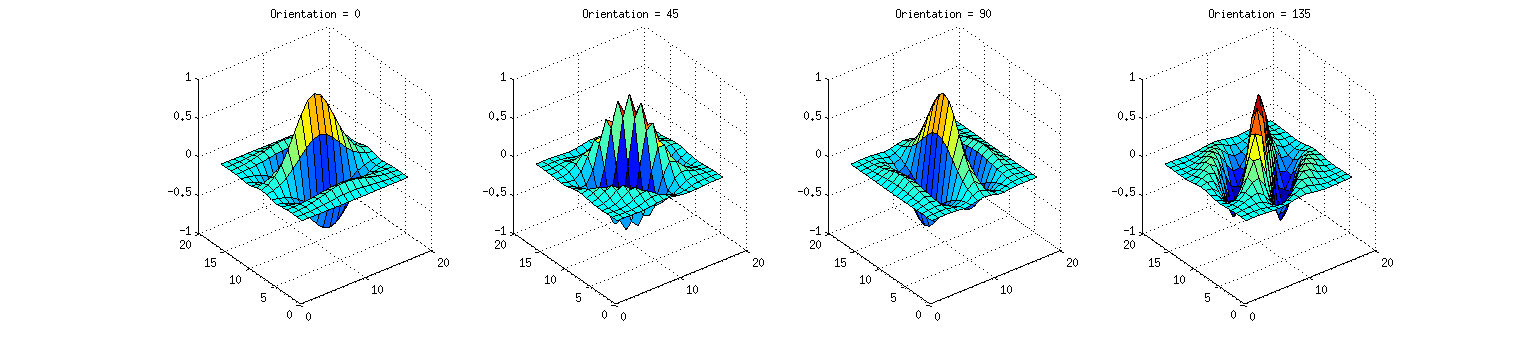
\includegraphics[width=0.95\textwidth]{pics/gabor.png}
	\caption{Real parts of the Gabor filters oriented to four directions.}
	\label{fig:gabor}
\end{figure*}

The templates (see Figure~\ref{fig:template}) are manually selected from the output of the pooling layer in the framed Matlab simulation. 
The output score of a convolution neuron is higher when its receptive field matches a certain template more. 
There are five populations of template matching neurons for five gestures in our system. 
The activity of the template matching populations indicates naturally the position of the gestures.

\begin{figure*}
\centering
	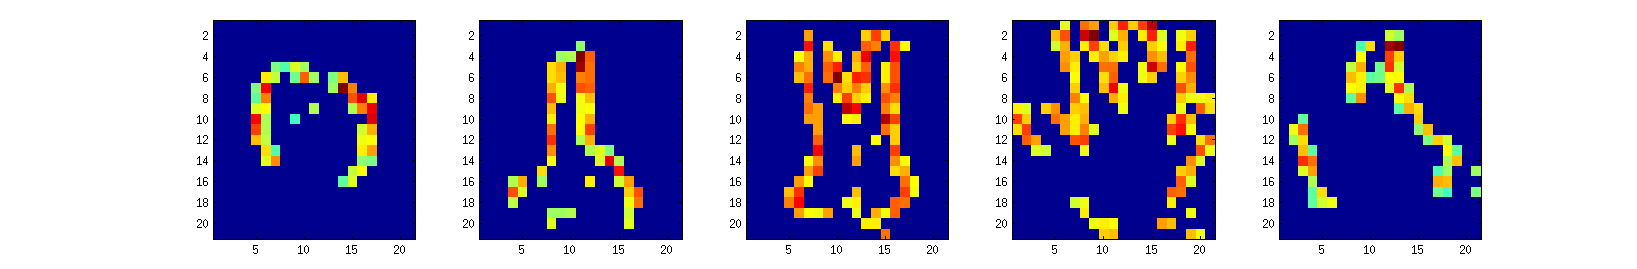
\includegraphics[width=0.95\textwidth]{pics/guesture.png}
	\caption{Five gesture templates}
	\label{fig:template}
\end{figure*}

\subsubsection{Combined Convolution Network}
Inspired by the research of Lecun~\cite{lecun1998gradient} and etc., we designed a combined network model with MLP and the convolutional network (Figure~\ref{fig:model2}). 
Thanks to the help of tracking, only the most active region in the pooling layer is forwarded to the next layer. 
A trained static 3-layered MLP is attached to classify the gesture.

\begin{figure}
\centering
	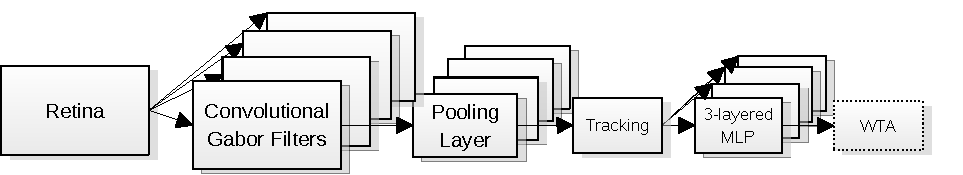
\includegraphics[width=0.42\textwidth]{pics/model2.pdf}
	\caption{The combined convolutional model with trained MLP neurons.}
	\label{fig:model2}
\end{figure}

Since the size of the input image of the MLP training is fixed and the position is centered, tracking plays a very important role to spot the valid region. 
Tracking is naturally embedded in the pooling layer of the convolutional network, for the active neurons directly point out the lively receptive field. 
\textcolor{red}{However, to extract only the active region to the next layer is still need to investigate.}

\subsection{Training and Testing}
\label{sec:tat}
Training is missing here.

In order to evaluate the cost and performance trade-offs in optimizing the number of neural components, both the convolutional models described above were tested at different sizes. 
Five gesture videos were captured from the silicon retina in address-event representation (AER~\cite{lazzaro1995multi}) format.  
All the gestures are of similar size and moving clock-wise in front of the retina. 
The videos are cut into frames (30ms/frame) and push forward into the convolutional networks. 
The configurations of the networks are listed in Table~\ref{tbl:nns} (Model 1: template matching; Model 2: trained MLP). 
The integration layer is not necessary in a convolutional network, it is used here to fit the template matching and decrease the number of synaptic connections.

\begin{table}
\caption{Sizes of the convolutional neural networks.}
	\begin{subtable}{0.5\textwidth}
		
		\centering
		\caption{Model 1: Template matching}
		\begin{tabular}{p{0.13\textwidth}|p{0.15\textwidth}<{\centering}|p{0.13\textwidth}<{\centering}|p{0.13\textwidth}<{\centering}|p{0.13\textwidth}<{\centering}}
		%Line 1
		\Xhline{1.2pt}
		    & \multicolumn{2}{c|}{\tabincell{c}{\textbf{Full} \\\textbf{Resolution}}}  
		    & \multicolumn{2}{c}{\tabincell{c}{\textbf{Sub-sampled} \\\textbf{Resolution}}}
		    \\ \cline{2-5}
		%Line 2
			& \tabincell{c}{Neuron \\ Number}
			& \tabincell{c}{Connections \\ per Neuron}
			& \tabincell{c}{Neuron \\ Number}
			& \tabincell{c}{Connections \\ per Neuron}
			\\ \Xhline{1.2pt}
		%Line 3
		\tabincell{l}{\textbf{Retinal} \\\textbf{Input}}
			& 128 $\times$ 128	& 1	& 32 $\times$ 32	& 4 $\times$ 4
			\\ \hline
		%Line 4
		\tabincell{l}{\textbf{Gabor} \\\textbf{Filter}}
			& 112$\times$112$\times$4	& 17 $\times$ 17	& 28$\times$28$\times$4	& 5 $\times$ 5
			\\ \hline
		%Line 5
		\tabincell{l}{\textbf{Pooling} \\\textbf{Layer}}
			& 36$\times$36$\times$4	& 5 $\times$ 5	& null	& null
			\\ \hline
		%Line 6
		\tabincell{l}{\textcolor[rgb]{0.55,0.55,0.55}{\textbf{Integration}} \\ \textcolor[rgb]{0.55,0.55,0.55}{\textbf{Layer}}}
			& 36 $\times$ 36	& 4	& 28 $\times$ 28	& 4
			\\ \hline
		%Line 7
		\tabincell{l}{\textbf{Template} \\\textbf{Matching}}
			& 16$\times$16$\times$5	& 21 $\times$ 21	& 14$\times$14$\times$5	& 15 $\times$ 15
			\\ \Xhline{1.2 pt}
		%Line 8
		\textbf{Total}
			& $74\,320$	& $15\,216\,512$	& $5\,925$	& $318\,420$
			\\ \Xhline{1.2 pt}
		\end{tabular}
		\label{tbl:m1}
	\end{subtable}
	\par\bigskip
	\begin{subtable}{0.5\textwidth}
		
		\centering
		\caption{Model 2: Trained MLP network layers after tracking}
		\begin{tabular}{p{0.13\textwidth}|p{0.15\textwidth}<{\centering}|p{0.13\textwidth}<{\centering}|p{0.13\textwidth}<{\centering}|p{0.13\textwidth}<{\centering}}
		%Line 1
		\Xhline{1.2pt}
		    & \multicolumn{2}{c|}{\tabincell{c}{\textbf{Full} \\\textbf{Resolution}}}  
		    & \multicolumn{2}{c}{\tabincell{c}{\textbf{Sub-sampled} \\\textbf{Resolution}}}
		    \\ \cline{2-5}
		%Line 2
			& \tabincell{c}{Neuron \\ Number}
			& \tabincell{c}{Connections \\ per Neuron}
			& \tabincell{c}{Neuron \\ Number}
			& \tabincell{c}{Connections \\ per Neuron}
			\\ \Xhline{1.2pt}
		%Line 3
		\tabincell{l}{\textbf{Tracked} \\\textbf{Input}}
			& 21 $\times$ 21	& null	& 15 $\times$ 15	& null
			\\ \hline
		%Line 4
		\tabincell{l}{\textbf{Hidden} \\\textbf{Layer}}
			& 10	& 21$\times$21$\times$10	& 10	& 15$\times$15$\times$10
			\\ \hline
		%Line 5
		\tabincell{l}{\textbf{Recognition} \\\textbf{Layer}}
			& 5	& 5$\times$10	& 5	& 5$\times$10
			\\ \Xhline{1.2pt}
		%Line 6
		\textbf{Total}
			& $456$	& $4\,460$	& $240$	& $2\,300$
			\\ \Xhline{1.2 pt}
		\end{tabular}
		\label{tbl:m2}
	\end{subtable}
	\label{tbl:nns}
\end{table}

\subsection{Experiment Results}
\label{sec:exp}

\begin{figure*}
\centering
	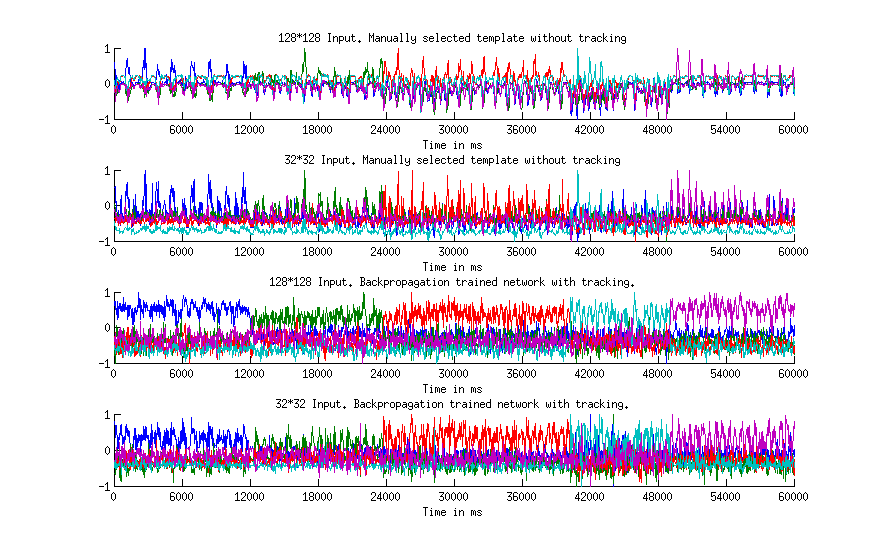
\includegraphics[width=0.9\textwidth]{pics/4.png}
	\caption{Neuron responses to the same five gesture videos.}
	\label{fig:matlabrec}
\end{figure*}




In Figure~\ref{fig:matlabrec} the first two plots refer to Model 1, using template matching. Each colour represents one of the recognition populations. 
Each point in the plot is the highest neuronal response in the recognition population during the time of one frame (30 ms). 
The neuronal response, the spiking rate, is normalized to [-1, 1]. 
It can be seen that the higher resolution input makes the boundaries between the classes clearer. 
On the other hand, recognition only happens when the test image and template are similar enough. 
The templates are only selected from the frames where the gestures are moving towards the right, and the gestures are moving clockwise in the videos. 
Thus, all the peaks in plot 1 signify that the direction of the gestures’ movement is right.  
It is notable that the higher resolution causes the recogniser to be more sensitive to the differences between the test data and the template, while the smaller neural network can recognize more generalized patterns. 
Therefore, a threshold is required to differentiate between data that is close enough and that which is not. 
Since the gestures are moving in four different directions during the clockwise movement, a rejection rate of 75\% is to be expected. 
The latter two plots refer to Model 2. 
The three-layer MLP network significantly improves the recognition rate and can generalize the pattern. 
There is no rejection rate for Model 2. 
The detailed results are listed in  Table~\ref{tbl:rsl}. 
The correct recognition rate is calculated from the non-rejected frames.
The lower resolution of the 32$\times$32 retina input is adequate for this gesture recognition task. 
The smaller network uses only 1/10 the number of neurons and 1/50 the number of synaptic connections compared to the full resolution network, while the recognition rate drops only around 10\% with Model 1 and 15\% with Model 2.

\begin{table}
\centering
\caption{Recognition results}
	\begin{tabular}{p{0.075\textwidth}|p{0.05\textwidth}<{\centering}|p{0.055\textwidth}<{\centering}|p{0.055\textwidth}<{\centering}|p{0.055\textwidth}<{\centering}|p{0.055\textwidth}<{\centering}}
		%Line 1
		\Xhline{1.2pt}
		    \multicolumn{2}{c|}{}	& \multicolumn{2}{c|}{\textbf{Model 1}}  
		    & \multicolumn{2}{c}{\textbf{Model 2}}
		    \\ \cline{3-6}
		%Line 2
		\multicolumn{2}{c|}{}	& \tabincell{c}{High \\ Resolution}
			& \tabincell{c}{Low \\ Resolution}
			& \tabincell{c}{High \\ Resolution}
			& \tabincell{c}{Low \\ Resolution}
			\\ \Xhline{1.2pt}
		%Line 3-4	
		\multirow{2}{*}{\tabincell{l}{\textbf{Fist} \\ (399 Frames)}}
			& Correct & 99.11\%	& 99.23\%	& 96.24\%	& 84.21\%
			\\ \cline{2-6}
			& Reject  & 71.93\% & 67.42\% 	& Null	& Null
			\\ \hline
		%Line 5-6
		\multirow{2}{*}{\tabincell{l}{\textbf{One Finger} \\ (392 Frames)}}
			& Correct & 92.98\%	& 80.00\%	& 94.39\%	& 71.69\%
			\\ \cline{2-6}
			& Reject & 70.92\%	& 75.77\% 	& Null	& Null
			\\ \hline
		%Line 7-8
		\multirow{2}{*}{\tabincell{l}{\textbf{Victory Sign} \\ (551 Frames)}}
			& Correct & 96.56\%	& 93.07\%	& 95.64\%	& 87.66\%
			\\ \cline{2-6}
			& Reject & 73.68\%	& 81.67\% 	& Null	& Null
			\\ \hline
		%Line 9-10
		\multirow{2}{*}{\tabincell{l}{\textbf{Full Hand} \\ (293 Frames)}}
			& Correct & 95.65\%	& 72.41\%	& 93.52\%	& 72.01\%
			\\ \cline{2-6}
			& Reject & 92.15\%	& 90.10\% 	& Null	& Null
			\\ \hline
		%Line 10-11
		\multirow{2}{*}{\tabincell{l}{\textbf{Thumb up} \\ (391 Frames)}}
			& Correct & 89.61\%	& 84.44\%	& 96.68\%	& 74.68\%
			\\ \cline{2-6}
			& Reject & 80.31\%	& 76.98\% 	& Null	& Null
			\\ \hline
	\end{tabular}
	\label{tbl:rsl}
\end{table}


\section{Real-Time Recognition on SpiNNaker}

\subsection{Moving from Rate-based to Spiking Neurons}
It remains a challenge to map the weights of a traditional artificial neural network to a spiking neural network. 
There are attempts to estimate the rate of Leaky integrate-and-fire (LIF) neurons with Poisson input spike trains~\cite{la2008response}. 
For the model illustrated above, there are two types of synaptic connection: one-to-one connections in the retina layer and N-to-one connections in all the convolutional layers (the pooling layer is also included). 
For the retina layer, 1) the problem is: what is the connection weight between two single LIF neurons to make a post-synaptic neuron fire whenever the pre-synaptic neuron generates a spike? 
While for the convolutional neurons, 2) given the input spike rates, LIF neuron parameters and the output spiking rate, what are the corresponding weights between the two layers?
\textcolor{blue}{In terms of the main goals of the report, the detailed mathematical reasoning will be demonstrated in the paper which will be submitted in November. 
A lot of work to be done here.}

\subsection{Live Recognition}
We implemented the prototype of the neural gesture recognition system on SpiNNaker. 
The input retina layer consists of 128$\times$128 neurons; 
each Gabor filter has 112$\times$112 valid neurons, since the kernel size is 17$\times$17; 
each pooling layer is as big as 36$\times$36, convolving with five template kernels (21$\times$21); 
thus, the recognition populations are 16$\times$16 neurons each. Altogether 74,320 neurons and 15,216,512 synapses use up to 19 chips on a 48-node board.

Figure~\ref{fig:live} shows snapshots of the real time gesture recognition system. Figure~\ref{fig:live1} is a snapshot of the Gabor filter layer, where Figure~\ref{fig:live2} shows the integration of all the pooled populations, and the active neurons in the visualizer in Figure~\ref{fig:live3} are pointing out the position of the recognized pattern (One finger). All the videos can be found on Youtube\footnote{\url{
http://youtu.be/PvJy6RKAJhw?list=PLxZ1W-Upr3eoQuLxq87qpUL-CwSphtEBJ, http://youtu.be/FZJshPCJ1pg?list=PLxZ1W-Upr3eoQuLxq87qpUL-CwSphtEBJ, http://youtu.be/yxN90aGGKvg?list=PLxZ1W-Upr3eoQuLxq87qpUL-CwSphtEBJ}}.

\begin{figure}
\centering
	\begin{subfigure}[t]{0.42\textwidth}
		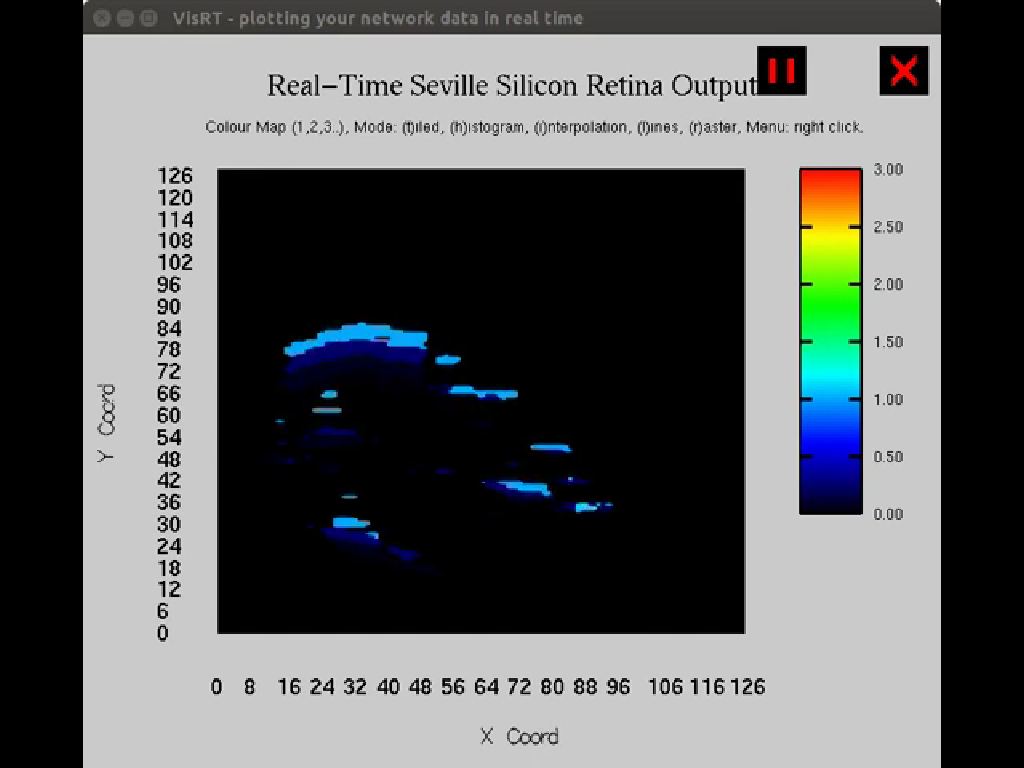
\includegraphics[width=\textwidth]{pics/live1.png}
	    \caption{Outline of the platform}
	    \label{fig:live1}
	\end{subfigure}
	\\
	\begin{subfigure}[t]{0.42\textwidth}
		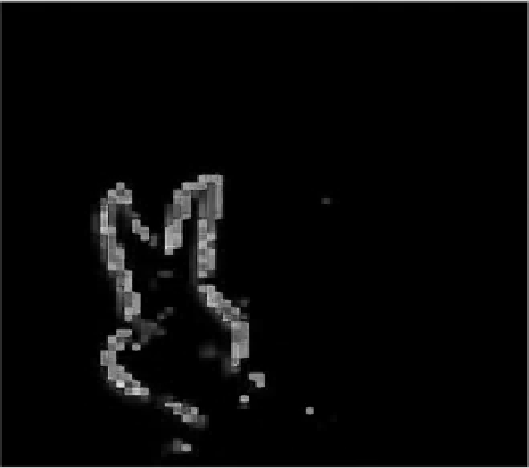
\includegraphics[width=\textwidth]{pics/live2.png}
		\caption{Picture of the hardware platform}
	    \label{fig:live2}
	\end{subfigure}
	\\
	\begin{subfigure}[t]{0.42\textwidth}
		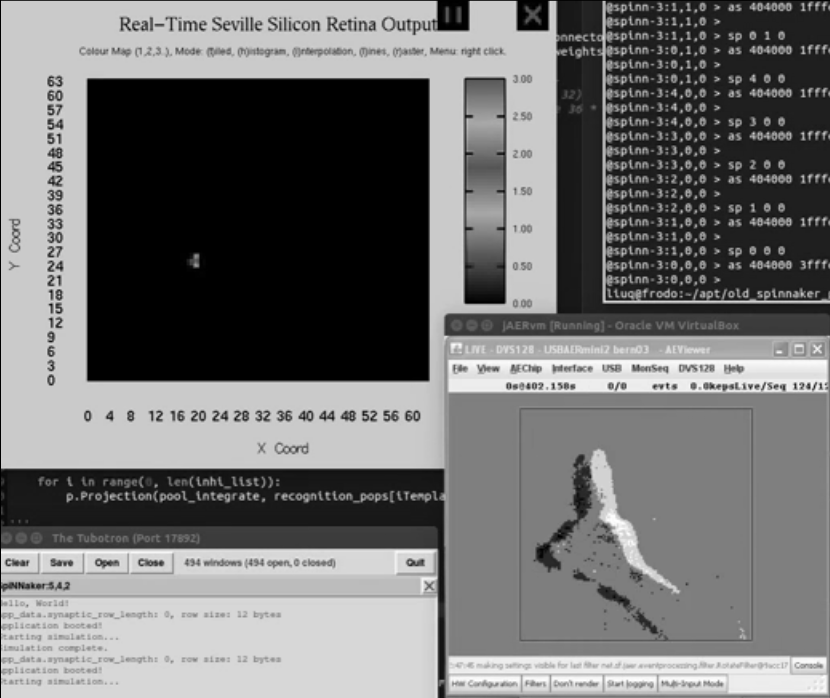
\includegraphics[width=\textwidth]{pics/live.png}
		\caption{Picture of the hardware platform}
	    \label{fig:live3}
	\end{subfigure}	

\caption{Snapshots of the real-time gesture recognition system on SpiNNaker.
}
\label{fig:live}
\end{figure}
  

\section{Plans and Prospects}
The future work will include more collaboration with biology and work with neuroscientist on vision systems, especially on the orientation detection region. 
To equip the system with tracking is another important job where the recognition performance will be increased and the short-term memory of a gesture route can be stored. Using the idea of HMMs to spiking neural networks may be a good approach. 
\bibliography{refs}    % this causes the references to be listed
\bibliographystyle{ieeetr}
\end{document}
